% AUTO-GENERATED by code/ch6_figs.py
\begin{tabular}{@{}r@{\hspace{8pt}}c@{\hspace{8pt}}l@{}}
input $\bm{x}$ & $\vcenter{\hbox{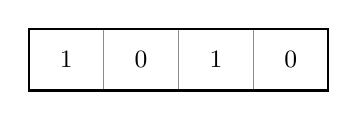
\begin{tikzpicture} \draw[black!45, fill=white] (0.000,0.000) rectangle (0.950,-0.779); \node[font=\small, text=black] at (0.475,-0.389) {$1$}; \draw[black!45, fill=white] (0.950,0.000) rectangle (1.900,-0.779); \node[font=\small, text=black] at (1.425,-0.389) {$0$}; \draw[black!45, fill=white] (1.900,0.000) rectangle (2.850,-0.779); \node[font=\small, text=black] at (2.375,-0.389) {$1$}; \draw[black!45, fill=white] (2.850,0.000) rectangle (3.800,-0.779); \node[font=\small, text=black] at (3.325,-0.389) {$0$}; \draw[line width=0.9pt] (0.000,0.000) rectangle (3.800,-0.779); \end{tikzpicture}}}$ & \tok{waste}\\[3pt]
square each entry & $\vcenter{\hbox{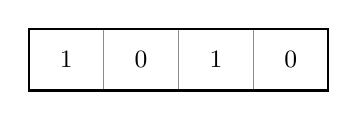
\begin{tikzpicture} \draw[black!45, fill=white] (0.000,0.000) rectangle (0.950,-0.779); \node[font=\small, text=black] at (0.475,-0.389) {$1$}; \draw[black!45, fill=white] (0.950,0.000) rectangle (1.900,-0.779); \node[font=\small, text=black] at (1.425,-0.389) {$0$}; \draw[black!45, fill=white] (1.900,0.000) rectangle (2.850,-0.779); \node[font=\small, text=black] at (2.375,-0.389) {$1$}; \draw[black!45, fill=white] (2.850,0.000) rectangle (3.800,-0.779); \node[font=\small, text=black] at (3.325,-0.389) {$0$}; \draw[line width=0.9pt] (0.000,0.000) rectangle (3.800,-0.779); \end{tikzpicture}}}$ & average of these $= 0.500$\\[3pt]
$\bm{x}/\RMS(\bm{x})$ & $\vcenter{\hbox{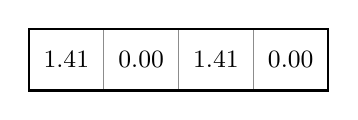
\begin{tikzpicture} \draw[black!45, fill=white] (0.000,0.000) rectangle (0.950,-0.779); \node[font=\small, text=black] at (0.475,-0.389) {$1.41$}; \draw[black!45, fill=white] (0.950,0.000) rectangle (1.900,-0.779); \node[font=\small, text=black] at (1.425,-0.389) {$0.00$}; \draw[black!45, fill=white] (1.900,0.000) rectangle (2.850,-0.779); \node[font=\small, text=black] at (2.375,-0.389) {$1.41$}; \draw[black!45, fill=white] (2.850,0.000) rectangle (3.800,-0.779); \node[font=\small, text=black] at (3.325,-0.389) {$0.00$}; \draw[line width=0.9pt] (0.000,0.000) rectangle (3.800,-0.779); \end{tikzpicture}}}$ & $\RMS = \sqrt{0.500} = 0.707$; divide every entry\\[3pt]
times gain $\bm{g}$ & $\vcenter{\hbox{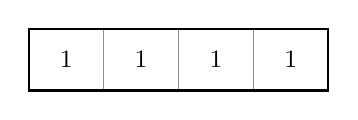
\begin{tikzpicture} \draw[black!45, fill=white] (0.000,0.000) rectangle (0.950,-0.779); \node[font=\small, text=black] at (0.475,-0.389) {$1$}; \draw[black!45, fill=white] (0.950,0.000) rectangle (1.900,-0.779); \node[font=\small, text=black] at (1.425,-0.389) {$1$}; \draw[black!45, fill=white] (1.900,0.000) rectangle (2.850,-0.779); \node[font=\small, text=black] at (2.375,-0.389) {$1$}; \draw[black!45, fill=white] (2.850,0.000) rectangle (3.800,-0.779); \node[font=\small, text=black] at (3.325,-0.389) {$1$}; \draw[line width=0.9pt] (0.000,0.000) rectangle (3.800,-0.779); \end{tikzpicture}}}$ & the toy's gain: all 1 (learned in real models)\\[3pt]
output & $\vcenter{\hbox{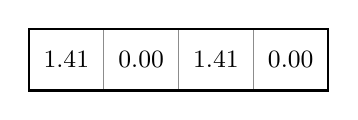
\begin{tikzpicture} \draw[black!45, fill=white] (0.000,0.000) rectangle (0.950,-0.779); \node[font=\small, text=black] at (0.475,-0.389) {$1.41$}; \draw[black!45, fill=white] (0.950,0.000) rectangle (1.900,-0.779); \node[font=\small, text=black] at (1.425,-0.389) {$0.00$}; \draw[black!45, fill=white] (1.900,0.000) rectangle (2.850,-0.779); \node[font=\small, text=black] at (2.375,-0.389) {$1.41$}; \draw[black!45, fill=white] (2.850,0.000) rectangle (3.800,-0.779); \node[font=\small, text=black] at (3.325,-0.389) {$0.00$}; \draw[line width=0.9pt] (0.000,0.000) rectangle (3.800,-0.779); \end{tikzpicture}}}$ & length $= 2.000 = \sqrt{d}$\\[3pt]
\end{tabular}
